% LaTeX document class and template packages
\documentclass[10pt,twocolumn,twoside]{article}
\usepackage[margin=0.75in]{geometry}
\usepackage{url}
\usepackage{color}
\usepackage{amsmath}
\usepackage{algorithm}
\usepackage{algorithmicx}
\usepackage{graphicx}
\usepackage[numbers,sort&compress,comma]{natbib}
\usepackage[colorlinks=true,linkcolor=blue,citecolor=blue,urlcolor=blue]{hyperref}
\usepackage{nameref} % nameref must be after hyperref
\usepackage{wrapfig}
\usepackage{hyperref}

% LaTeX document preamble and commands
\newcommand{\etal}{\textit{et al.}}
\pagestyle{myheadings}
\date{} % filename BHAVI2016JLCT.tex
\author{Jason~J.~Liu, Daniel~Yang, Adam~Craig, and Carl~Taswell}
\title{Using MongoDB and Mongoose with a MEAN Stack Implementation of the NEXUS-PORTAL-DOORS System\\ } 
\markboth{J.~J.~Liu \etal}{BHA-2016-06 ver \today}

% LaTeX document
\begin{document}
\maketitle
\thispagestyle{empty}

\section*{Introduction}
\label{secIntroduction}
	For researchers, primary research is only the first stepping stone to proving or disproving a hypothesis. One successful experiment proves little to nothing in the grand scheme of the scientific community. However, the weakness of a single experiment is covered by the power of the meta-analysis, usually completed by a third party. Meta-analysis requires researchers to analyze results from muliple primary articles and assess whether or not the result is accurate, show if the hypothesis presented are proven or disproven, and provide a degree of error. However, despite the necessity of meta-analyses, it continues to be time consuming and ineffective at connecting with all points of data. The miniscule amount of secondary articles pale in comparison to the literal thousands of primary articles which are published each day. In order to take advantage of all the new information which is provided and to create more effective secondary analyses, a semantic web solution provides the necessary tools in order to take full statistical advantage that meta-analysis offers. 
 \newline
	One such implementation of a meta-analysis system is the NEXUS-PORTAL-DOORS (NPD) system. In order to support PORTAL registries and DOORS directories, a database is necessary in order to support and store the data. In order to take full advantage of a tried and true framework, MEAN stack serves as the ideal system by thoroughly integrating client-side, server-side, and database processes. As part of that stack, MongoDB alongside Mongoose enables a heirarchical database for storing resource metadata 

\section*{Methods}

\label{secMethods}

\iffalse
\begin{wrapfigure}[15]{r}{4in}
\centering
 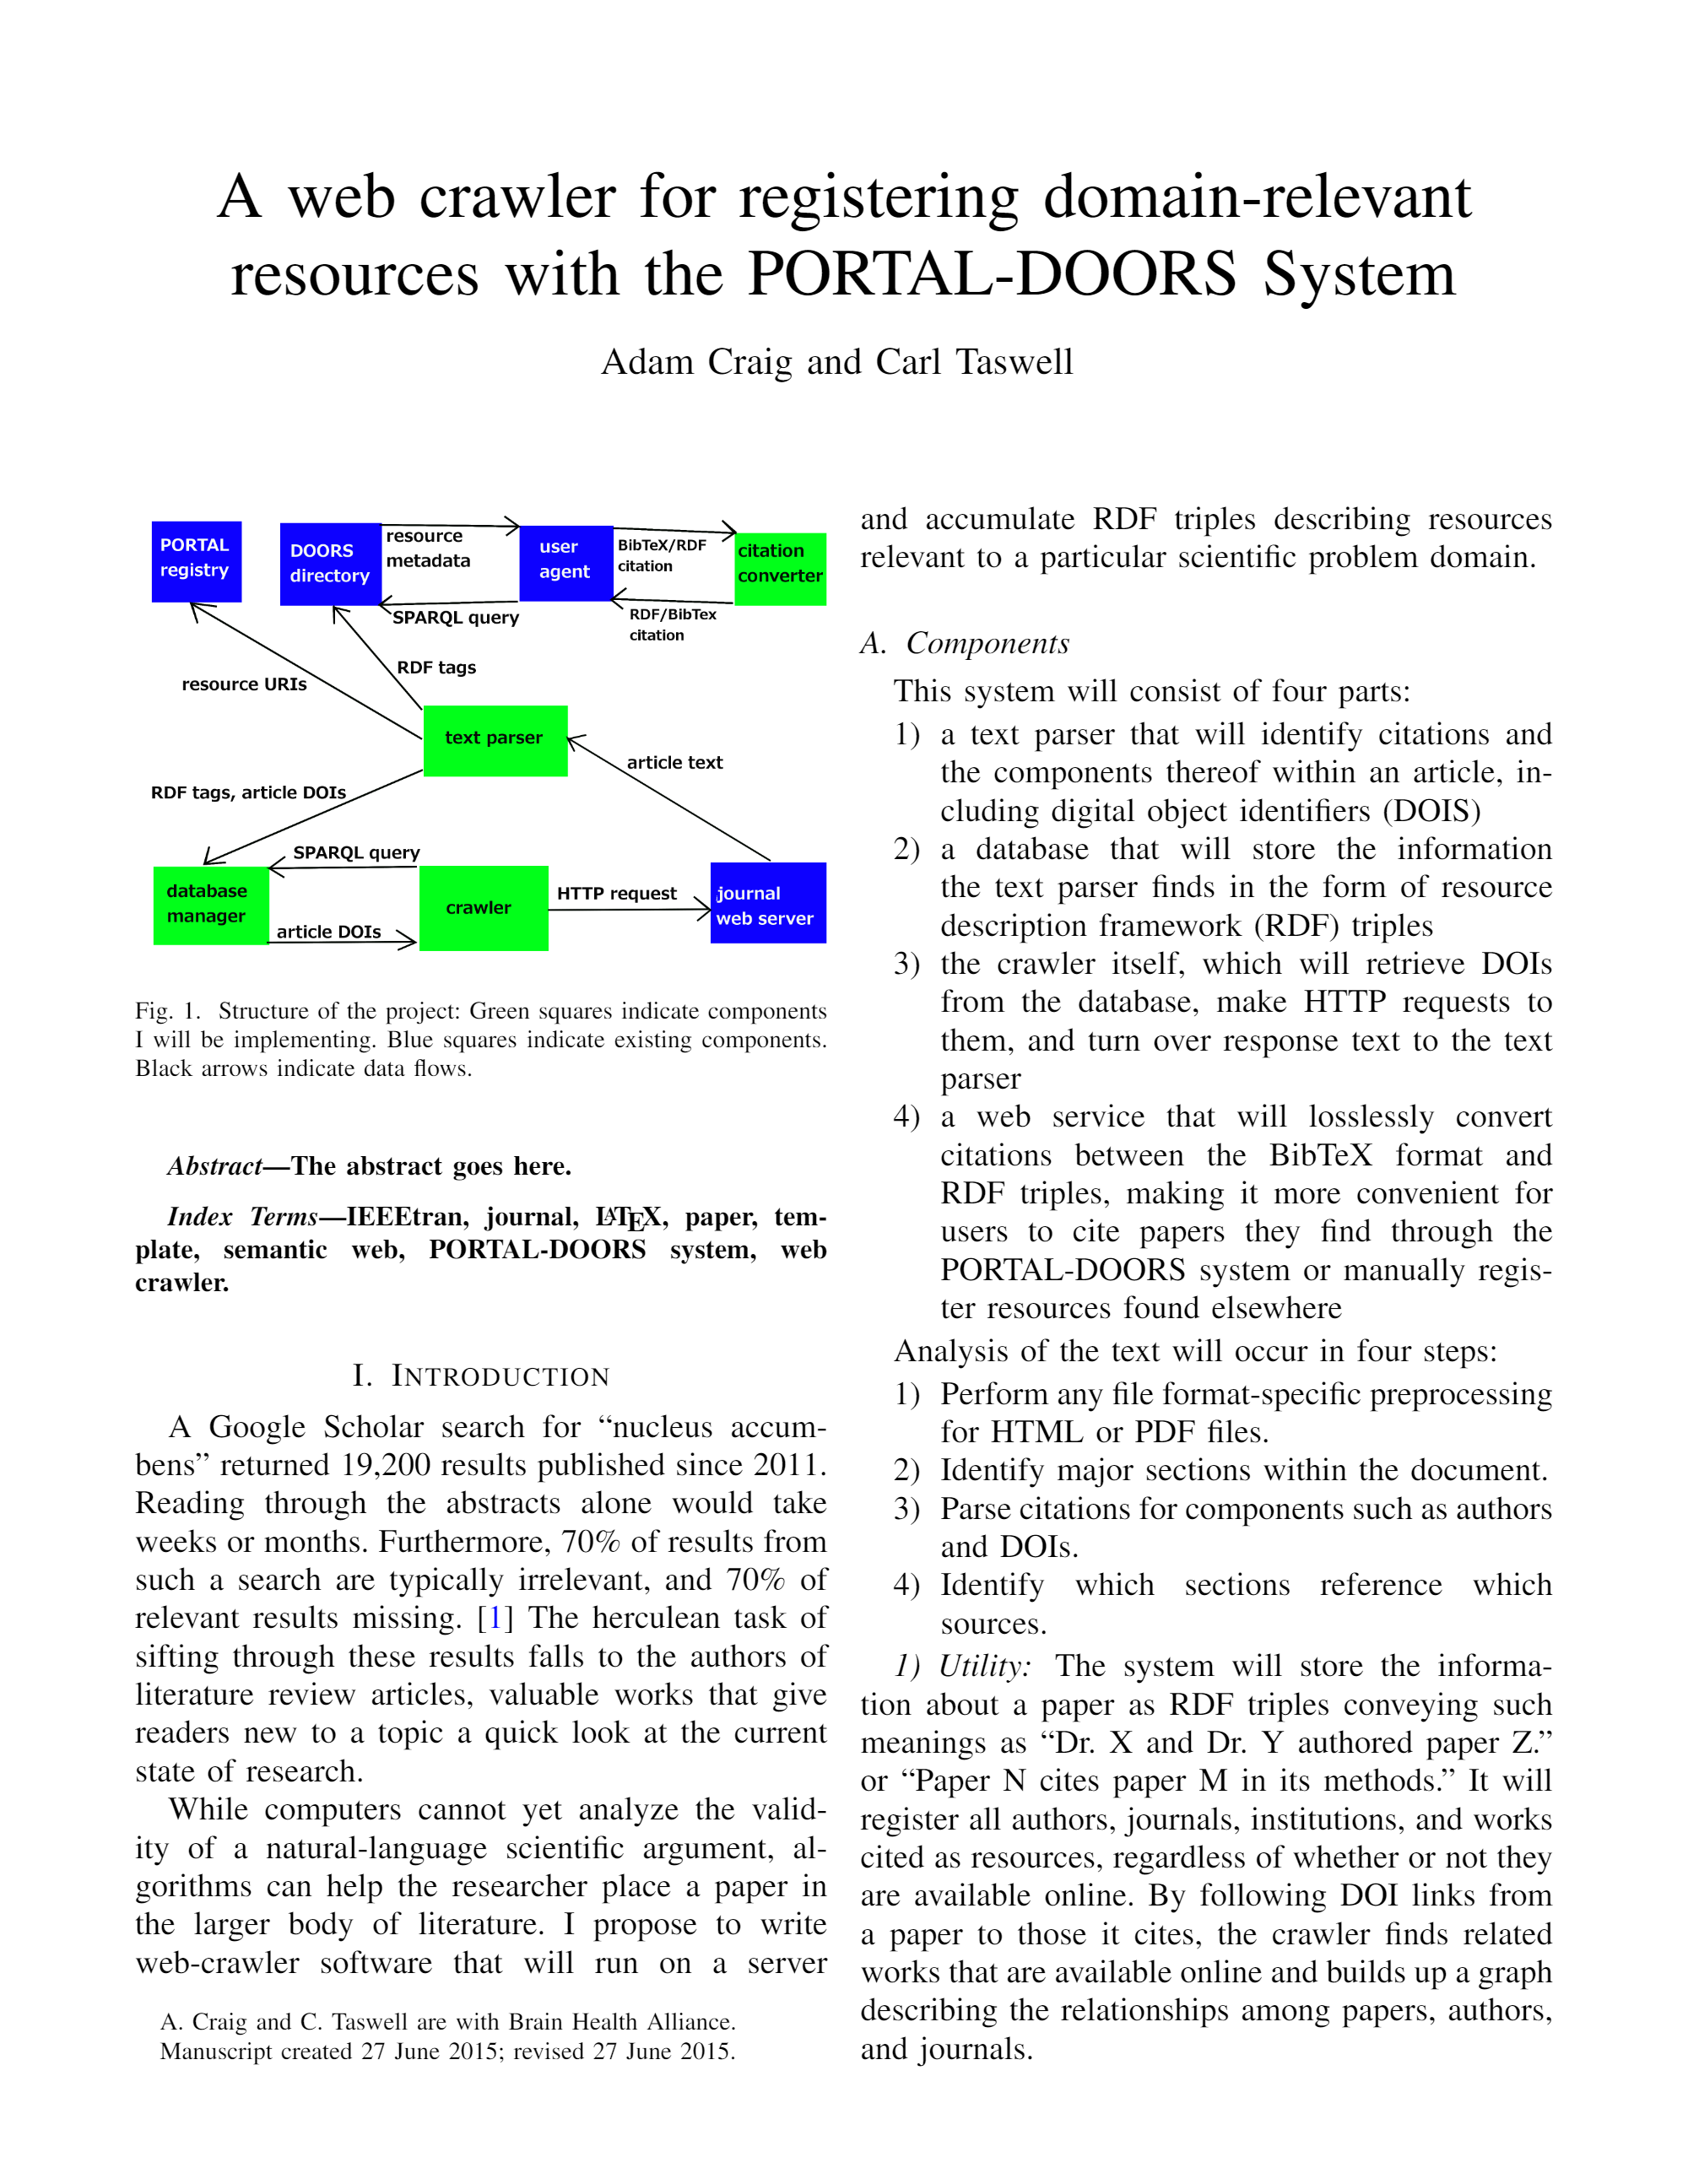
\includegraphics[scale=0.35]{NPDS_flowchart}	
\end{wrapfigure}
\fi

	For this new NEXUS-PORTAL-DOORS (NPD) system implementation, MEAN (MongoDB, Express, Angular, Node.js)  stack is the most updated and contributed fullstack javascript framework. Both backend and front end will rely heavily on node.js, an open-source runtime environment which enables scalable web applications and servers. Used with Express and other packages, node.js enables the user to organize a web application into a MVC (model-view-controller) architecture. In accordance with the "M" from MEAN stack, MongoDB serves as the database for the NPD. As a noSQL database, MongoDB relies on collecetions and documents in contrast to tables and rows. However, MongoDB offers no implementation of queries or updates to the database. Mongoose, a popular object relational mapper for MongoDB, enables connection to a MongoDB database from javascript, allowing model abstraction, large scale queries, data validation, and more. It also enables the user to create schemas, which help generate a structured database. \newline
	
	In the NPDS system, Problem Oriented Registry of Tags And Labels (PORTAL) registers resource labels and tags, inserting or updating them into the database while the Domain Ontology Oriented Resource System (DOORS) publishes resource locations and descriptions with mapping of labels to locations for the semantic web, retrieving stored data from the database. Both PORTAl and DOORS can be optimized for faster read/write if organized in a heirarchical architecture organized through XML. Within the database, the collections for each of these PORTAL, DOORS, AND NEXUS are named respectively with the prefixes pds P, pds D, and pds N. The database schema for these collections contains a String identifier and a javascript Object, where the JSON converted from XML is stored. The identifer is a tag which helps queries traverse and retreive the correct resource while the Object contains:\newline

\begin{itemize}
  \item Resource Entity: 
  \item Resource Record:
  \item Resource Infoset: 
  \item Resource Representation:
  \item Resource Messages: 
\end{itemize}
	In the previous implementation of NPDS, the Microsoft SQL database contained resources in lengthy tables with each column containing a small piece of information which would be used to build an XML document. However, MongoDB's documentless database structure enables the same metadata resource information to be kept in XML format. However, XML format is not supported by any databases, including Mongoose/MongoDB. Terefore, it is necessary to convert the XML into a data type which is recognized by Mongoose and able to be stored by MongoDB, of which JSON is the most reliable. In order to translate between XML is JSON, xml2js is used for XML to JSON conversion and easyxml for JSON to XML conversion.  \newline

	It is also vital that NEXUS, PORTAL, and DOORS sections of the NPDS system be able to communicate with one another. By using Mongoose, the schema of a collection can be modeled to point at another collection. Combined with queries, this enables a user to communicate and exchange information between NEXUS, PORTAL, and DOORS.  \newline

	In order to create this implementation of MongoDB and Mongoose for a NPDS system, a template is required as the starting platform. Working with other parts of the NPDS implementation, MongoDB will serve two purposes. One is to contain users for an authentication system, working alongside PassportJS. PassportJS enables the creation of accounts under username and password. It can also be implemented to receive authentication from third parties sucha s Facebook and Twitter, a common practice nowadays. However, for our purposes, the primary advantage of using passport is the level of flexibility it offers. Its primary goal is to keep the complexity of user authentication simple and done in as a few lines of code as possible. This is done with "strategies," which are modules which enable the user to specifically designate which form of authentication they desire, without uncessary modules. PassportJS also supports persistent sessions. Lastly, PassportJS enables the database to store the username as a string, but encodes the password with a series of numbers, ensuring a level of security for the user. The second purpose of MongoDB in the template is to read/write/store metadata. Although the collection names will be changed upon the generation of each server from the template, the role will not. The pimary purpose of the database in the PORTAL registrar is to be able to store metadata resources with labels and optional tags. Meanwhile, the in the DOORS directories, the database must be able to retrieve locations and descriptions of resources, which are specified by references to an OWL ontology.

August:
\begin{itemize}
	\item Week 4: Finish javascript fo creating and inserting xml into MongoDB, presentation
\end{itemize}
	

\section*{Results}
	The implementation of MongoDB for NPDS is a partial success. Currently, writing to the registrar is done smoothly in Mongoose. Storing XML data is also a success, being enabled by the npm module xml2js. However, retrievel through queries is currently still an issue. 


\section*{Discussion}
	Due to the flexbility of noSQL and especially lMongoDB's document based database, it offers a database storage which fit the purposes of storing metadata. Furthermore, the automation of this process is enabled by Mongoose, which also helps create a schema and acts as an ORM. The currently implementation proves the potential for a noSQL database such as MongoDB to play a role in the future of NPDS or other semantic web systems. 


\section*{Conclusion}
\label{secConclusion}
conclusion text here


\section*{Acknowledgments}
This research was supported by the Brain Health Alliance Virtual Institute. We'd like to thank everyone who particpated in the 2016 program with us, especially Sujay Ratna and Ben Bae, who worked with us toward a semantic web solution. 


\section*{References}
\begin{enumerate}
\item Cattell, R.
Scalable SQL and NoSQL data stores \href{https://scholar.google.com/scholar?q=Scalable+SQL+and+NoSQL+data+stores&btnG=&hl=en&as_sdt=0%2C47}{[Google Scholar]}

\item Daniel Peng Frank Dabek, G. I.
Large-scale Incremental Processing Using Distributed Transactions and Notifications
 \href{https://scholar.google.com/scholar?q=Large-scale+Incremental+Processing+Using+Distributed+Transactions+and+Notifications&btnG=&hl=en&as_sdt=0%2C47}{[Google Scholar]}

\item Elif Dede Daniel Gunter, R. S. C. L. R.
Performance evaluation of a mongodb and hadoop platform for scientific data analysis
 \href{https://scholar.google.com/scholar?q=Performance+evaluation+of+a+mongodb+and+hadoop+platform+for+scientific+data+analysis&btnG=&hl=en&as_sdt=0%2C47}{[Google Scholar]}

\item Ghislain Fourny Jsoniq The, S. N. G. F.
JSONiq The SQL of NoSQL
 \href{http://citeseerx.ist.psu.edu/viewdoc/summary?doi=10.1.1.366.3332}{[Google Scholar]}

\item Harpinder Kaur, J. S.
Improvement in Load Balancing Technique for MongoDB Clusters
 \href{https://scholar.google.com/scholar?q=Improvement+in+Load+Balancing+Technique+for+MongoDB+Clusters&btnG=&hl=en&as_sdt=0%2C47}{[Google Scholar]}

\item Jyotsna Talreja Wassan, A. P.
Exploratory Implementation of Stream Clustering Algorithm using MongoDB
 \href{https://scholar.google.com/scholar?q=aExploratory+Implementation+of+Stream+Clustering+Algorithm+using+MongoDB&btnG=&hl=en&as_sdt=0%2C47}{[Google Scholar]}

\item Ljiljana Stojanovic Nenad Stojanovic, R. V.
Migrating data-intensive Web Sites into the Semantic Web
 \href{https://scholar.google.com/scholar?q=Migrating+data-intensive+Web+Sites+into+the+Semantic+Web&btnG=&hl=en&as_sdt=0%2C47}{[Google Scholar]}

\item Pradeep Soni, N. S. Y.
Quantitative Analysis of Document Stored Databases
 \href{https://scholar.google.com/scholar?q=Quantitative+Analysis+of+Document+Stored+Databases&btnG=&hl=en&as_sdt=0%2C47}{[Google Scholar]}

\item Rajat Aghi Sumeet Mehta, R. C. S. C. N. B.
A comprehensive comparison of SQL and MongoDB
 \href{https://scholar.google.com/scholar?q=A+comprehensive+comparison+of+SQL+and+MongoDB&btnG=&hl=en&as_sdt=0%2C47}{[Google Scholar]}

\item Rupali Arora, R. R. A.
Modeling and Querying Data in MongoDB
 \href{https://scholar.google.com/scholar?q=Modeling+and+Querying+Data+in+MongoDB&btnG=&hl=en&as_sdt=0%2C47}{[Google Scholar]}

\item Sanobar Khan, P. V. M.
SQL Support over MongoDB using Metadata
 \href{https://scholar.google.com/scholar?q=SQL+Support+over+MongoDB+using+Metadata&btnG=&hl=en&as_sdt=0%2C47}{[Google Scholar]}

\item Stefanie Scherzinger, M. K.
Managing Schema Evolution in NoSQL Data Stores
 \href{https://scholar.google.com/scholar?q=Managing+Schema+Evolution+in+NoSQL+Data+Stores&btnG=&hl=en&as_sdt=0%2C47}{[Google Scholar]}

\item Taswell, C.
Correction Corrections to “DOORS to the Semantic Web and Grid With a PORTAL for Biomedical Computing”
2008
 \href{https://scholar.google.com/scholar?q=Correction+Corrections+to+%E2%80%9CDOORS+to+the+Semantic+Web+and+Grid+With+a+PORTAL+for+Biomedical+Computing%E2%80%9D&btnG=&hl=en&as_sdt=0%2C47}{[Google Scholar]}

\item Taswell, C.
DOORS to the semantic web and grid with a PORTAL for biomedical computing
2008
 \href{https://scholar.google.com/scholar?q=Correction+Corrections+to+%E2%80%9CDOORS+to+the+Semantic+Web+and+Grid+With+a+PORTAL+for+Biomedical+Computing%E2%80%9D&btnG=&hl=en&as_sdt=0%2C47}{[Google Scholar]}

\item Taswell, C.
Article A Distributed Infrastructure for Metadata about Metadata: The HDMM Architectural Style and PORTAL-DOORS System
2010 \newline
\href{http://www.mdpi.com/1999-5903/2/2/156/htmg}{[MDPI]} 

\item Zhengxiang Pan, J. H.
DLDB: Extending Relational Databases to Support Semantic Web Queries
2003
\href{https://scholar.google.com/scholar?hl=en&q=DLDB%3A+Extending+Relational+Databases+to+Support+Semantic+Web+Queries&btnG=&as_sdt=1%2C47&as_sdtp=}{[Google Scholar]}

\item Dickey, J.
Write modern web apps with the MEAN stack: Mongo, Express, AngularJS, and Node. js
Education, P. (ed.)
Pearson Education, 2014
 \href{}{[Google Scholar]}

\item Pasquali, S.
Mastering Nodejs
Edward Gordan, G. W. (ed.)
Packet Publishing Ltd., 2013
 \href{}{[Google Scholar]}

\item Chodorow, K. and Dirolf, M.
MongoDB: The Definitive Guide
Steele, J. (ed.)
O' Reilly, 2010
 \href{}{[Google Scholar]}

\item Holmes, S.
Mongoose for Application Development
Mizen, G. (ed.)
Packet Publishing Ltd., 2013
 \href{}{[Google Scholar]}

\item Barrasa Rodriguez J., C. �.. and G�mez-P�rez, A.
R2O, an extensible and semantically based database-to-ontology mapping language
Springer-Verlag, 2004
 \href{}{[Google Scholar]}

\item Kei-Hoi Cheung Andrew K. Smith, K. Y. Y. C. J. B. and Gerstein, M. B.
Semantic Web Approach to Database Integration in the Life Sciences
Revolutionizing Knowledge Discovery in the Life Sciences, 2007
 \href{}{[Google Scholar]}

\end{enumerate}


% References: note that the \nocite{*} command will automatically generate 
%  a reference list for all references contained in all *.bib files separated by
%  commas in the \bibliography{} command.
\nocite{*}
\bibliographystyle{plainnat}
\bibliography{BrainWarping}
\end{document}